\documentclass[varwidth=true, border=2pt]{standalone}

\usepackage{pgfplots}
\usepackage{tikz}

\begin{document}
	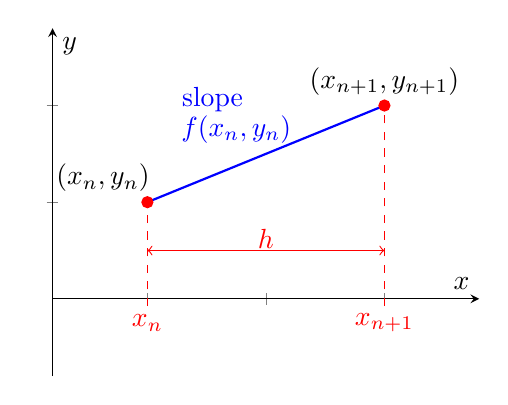
\begin{tikzpicture}
    \begin{axis}[
        legend pos=south east,
        axis x line=middle,
        axis y line=middle,
	xticklabels=\empty,
	yticklabels= \empty,
        grid = none ,
        width=7cm,
        height=6cm,
        grid style={dashed, gray!1},
        xmin=1,     % start the diagram at this x-coordinate
        xmax= 7,    % end   the diagram at this x-coordinate
        ymin=-1,     % start the diagram at this y-coordinate
        ymax= 5,   % end   the diagram at this y-coordinate
        xlabel=$x$,
        ylabel=$y$,
        enlargelimits=true,
        tension=0.08]

  \addplot[red, only marks, mark=*] coordinates {(2,2)(6,4)};
 % \draw [red,dashed] (axis cs: -0.1,2) -- (axis cs: 2,2);
  \draw [red, <->] (axis cs:2,1) -- (axis cs: 6,1);
  \draw [red,dashed] (axis cs: 2,-0.15) -- (axis cs: 2,2);
  \draw [red,dashed] (axis cs: 6,-0.15) -- (axis cs: 6,4);
  \draw[blue,thick](axis cs: 2,2)--(axis cs: 6,4);
      
	\node(c1) at (axis cs: 1.25, 2.5){$(x_n, y_n)$};
	\node(c2) at (axis cs: 6, 4.5){$(x_{n+1}, y_{n+1})$};
	\node(s1) [blue] at (axis cs: 3.5, 3.5){$f(x_n, y_n)$};
	\node(s2) [blue] at (axis cs: 3.1, 4.125){slope};
	\node(x1)[red] at (axis cs: 2,-0.5){$x_n$};
	\node(x2)[red] at (axis cs: 6,-0.5){$x_{n+1}$};
	\node(H) [red] at (axis cs: 4, 1.25){$h$};

    \end{axis}
\end{tikzpicture}
\end{document}